\documentclass[runningheads,orivec]{llncs}
\usepackage[T1]{fontenc}
\usepackage{lmodern}
\usepackage{amsmath,booktabs,graphicx,microtype,tikz,flafter}
\usepackage[section]{placeins}
\usetikzlibrary{arrows.meta,positioning}
\usepackage{xurl}
\usepackage[hidelinks]{hyperref}
\providecommand{\doi}[1]{\url{https://doi.org/#1}}
\hypersetup{
  pdftitle={Interpolation vs. Generalization in SAR Water Segmentation: An Event-Held-Out Study on Sen1Floods11 with an Azerbaijan Mapping Prototype},
  pdfauthor={Ali Agabalazade, Nigar Rustamova, Jala Suleymanova, Isgandar Panahov},
  pdfsubject={Original manuscript content licensed under CC BY 4.0; third-party material excluded}
}
\raggedbottom
\setlength{\tabcolsep}{5pt}
\begin{document}
\title{Interpolation vs. Generalization in SAR Water Segmentation: An Event-Held-Out Study on Sen1Floods11 with an Azerbaijan Mapping Prototype}
\titlerunning{Interpolation vs. Generalization in SAR Water Segmentation}
\author{Ali Agabalazade\inst{1} \and Nigar Rustamova\inst{1} \and
Jala Suleymanova\inst{2} \and Isgandar Panahov\inst{1}}
\authorrunning{A. Agabalazade et al.}
\institute{Azerbaijan State University of Economics (UNEC), Baku, Azerbaijan
\and Azerbaijan Technical University, Baku, Azerbaijan}
\maketitle

\begin{abstract}
Synthetic aperture radar (SAR) sees through clouds, which makes Sentinel-1
a natural sensor for rapid flood mapping. Segmentation models are usually
scored on chip-level splits whose test chips can come from the same flood
events as the training chips. We study how this within-event setting
differs from transfer to a new event on Sen1Floods11. The original
generalist comparison reused training and validation chips. We reconstruct a
paired official-test comparison of event-excluded DeepLabV3+/ResNet-50
checkpoints against a fixed seed-42 generalist on identical chips and valid
pixels. Nine of 30 planned event--seed pairs are recoverable, spanning
seven events and 51 unique paired chips. Five pooled water-IoU differences are
positive and four negative, ranging from $-0.0336$ to $+0.0253$. Omitting
one test chip can reverse the sign in seven of nine pairs. These results
describe the surviving checkpoints and observed test chips. Separately, we
present a SegFormer-B4 mapping prototype that combines JRC water occurrence
and terrain/coverage masks. The two unlabeled Azerbaijan scenes show
how filtering changes the map. Inundation accuracy remains unmeasured.
\keywords{SAR water segmentation \and event-held-out evaluation \and Sentinel-1}
\end{abstract}

\section{Introduction}
\label{sec:intro}

Floods are among the most frequent and damaging natural hazards, and timely
inundation maps are needed most while the storm is still overhead. Optical
imagery is often unusable at exactly that moment because of cloud cover.
Synthetic aperture radar (SAR) does not have this limitation. The Sentinel-1
mission delivers C-band SAR acquisitions day and night and through cloud
\cite{torres2012}. Open water often appears dark because smooth water surfaces
scatter the signal away from the sensor \cite{twele2016sentinel1}. This has
made Sentinel-1 a workhorse of operational flood mapping.

Deep segmentation networks trained on the Sen1Floods11 benchmark
\cite{bonafilia2020} are a strong data-driven alternative to threshold-based
processing chains. The standard evaluation, however, is a chip-level split
in which training and test chips can originate from the same flood events.
Scores obtained this way describe how well a model interpolates within
events it has already seen. What a practitioner needs to know is whether
the model generalizes to an event that contributed no training labels at
all. This matters for regions such as Azerbaijan that are absent from
Sen1Floods11.

We therefore use a leave-one-event-out protocol, retaining the historical
LOCO (leave-one-country-out) identifier. Each Sen1Floods11 hand-labeled
group corresponds to a flood event, so an excluded group represents a
particular event and region. A raw held-out IoU is hard to interpret on its
own, because some events are simply harder than others. We compare the
available event-excluded checkpoints with a fixed generalist on exactly
the same official test chips. This pairs the evaluation inputs while
leaving differences between the training and validation designs
(Sec.~\ref{sec:paired}).

Segmentation alone is also insufficient for a usable inundation map.
Wind-roughened water can look like land, recurrent water bodies look like
flood water, and SAR terrain distortions such as layover and shadow can
produce false detections. We address the last two with a post-processing
fusion that combines the JRC Global Surface Water layer \cite{pekel2016high}
with a DEM-derived terrain and coverage mask, separately from the
benchmark (Sec.~\ref{sec:fusion}).

\paragraph{Contributions.}
\begin{itemize}
\item We reconstruct a paired, official-test comparison on seven
Sen1Floods11 events and nine recoverable event--seed combinations
(Secs.~\ref{sec:dataset} and \ref{sec:loco}).
\item We report the seed-specific difference and show how it changes
when individual test chips are omitted (Sec.~\ref{sec:sensitivity}).
\item We document the VV/VH/ratio input, weak-to-hand training, and an
11-variant loss sweep under class imbalance
(Secs.~\ref{sec:method} and \ref{sec:ablations}).
\item We describe the prototype's recurrent-water and terrain/coverage
filters and their effect on two unlabeled Azerbaijani scenes
(Sec.~\ref{sec:deployment}).
\end{itemize}

\section{Related Work}
\label{sec:related}

\paragraph{SAR flood mapping.}
Classical Sentinel-1 flood mapping relies on automated thresholding and
change detection chains \cite{twele2016sentinel1}. Learning-based methods
became practical with georeferenced training data. Sen1Floods11
\cite{bonafilia2020} provides hand-labeled and weakly labeled Sentinel-1
chips from flood events on several continents and is the benchmark we
build on.

\paragraph{Ancillary layers and terrain effects.}
The JRC Global Surface Water dataset \cite{pekel2016high} records how often
each pixel has been observed as water over several decades and provides a
prior for recurrent water. On the SAR side, steep terrain produces layover
and shadow, whose extent depends on the viewing geometry and the local
slope. The same geometry underlies radiometric terrain correction
\cite{small2011}. Elevation data such as the Shuttle Radar Topography
Mission \cite{farr2007} make these effects computable per pixel.

\paragraph{Evaluating generalization.}
Random splits of spatially autocorrelated data can overestimate
performance on new locations, motivating blocked or leave-one-group-out
validation \cite{roberts2017}. T{\"u}rkmenli, Kayabol and Aptoula
\cite{turkmenli2025} treat flood events as source domains for
domain-generalization training, whereas we compare an event-excluded
checkpoint with a fixed generalist on that event's same official test
chips.

\paragraph{Segmentation under class imbalance.}
Water pixels are a small minority. Overlap-based objectives such as Dice
\cite{milletari2016}, Tversky \cite{salehi2017} and Focal-Tversky
\cite{abraham2019}, the Lov\'asz surrogate for IoU \cite{berman2018},
and focal loss \cite{lin2017focal} are common answers. We compare them
with weighted cross-entropy in a validation sweep (Sec.~\ref{sec:ablations}).

\section{Dataset and LOCO Protocol}
\label{sec:dataset}

\subsection{Sen1Floods11}

We use Sen1Floods11 \cite{bonafilia2020}, which provides $512\times512$
Sentinel-1 chips with labels from two sources. The hand-labeled subset
covers 11 flood events named by country or region, including the Mekong.
It contains 446 chips. Of these, 431 are in the standard split and 15
Bolivia chips are held out separately by design. The paired comparison
uses the ten standard groups and leaves out the separate Bolivia hand
holdout. The standard split has 252 training, 89 validation and 90 test
chips. The training share is 58.47\% of 431.

A much larger weakly labeled subset has labels derived automatically from
Sentinel-2 imagery. Bonafilia et al. report 4,385 weakly labeled chips.
The local manifests contain 4,384, with 3,946 train and 438 validation
entries across 12 filename groups, including Bolivia and Colombia. The
reason for the one-chip difference is unknown.

Water makes up 9.51\% of labeled pixels with finite SAR in the official
hand training split and 12.30\% in the official test split. The historical
10.6\% figure describes the full hand inventory. The labels mark water
present on the flood date, including both flood and persistent water.
This determines which model output can be scored (Sec.~\ref{sec:fusion}).

\subsection{Leave-One-Event-Out Protocol}
\label{sec:protocol}

For each planned fold, the reconstructed manifests remove the named
event from the hand and weak training and validation roles. Hand training
then uses 211--242 chips and hand validation uses 75--85. Three planned
seeds (42, 43 and 44) for the ten standard groups give 30 event--seed
combinations. The surviving runs cover only part of this design
(Sec.~\ref{sec:loco}).

The October reconstruction froze completed runs and their
checkpoints with the best validation IoU before paired inference. Committed
manifests, file hashes, run paths and validation histories support the
reconstruction of historical membership and checkpoint selection.
Runtime records of actual file reads and full initializer lineage were
unavailable, including the USA retry's exact pretraining initializer.

\subsection{Seed-Specific Paired Difference}
\label{sec:paired}

The original comparison scored the generalist across all 431 standard
hand chips, including the 252 used for hand training and 89 used for
validation. This mixed training, checkpoint-selection and test performance.
We now compare an event-excluded checkpoint for seed $s$ with a fixed
generalist of the same architecture and define
\begin{equation}
\Delta(e,s)=\operatorname{IoU}(\mathrm{LOCO}_{e,s},T_e)
             -\operatorname{IoU}(G_{42},T_e).
\label{eq:paired}
\end{equation}
Here $T_e$ contains only event $e$'s official test chips and $G_{42}$ is
the same seed-42 generalist checkpoint throughout. We use the same valid
mask in both arms, excluding ignored labels and non-finite SAR, and score
sigmoid probabilities strictly greater than 0.5 without test-time
augmentation or fusion. For each arm, water-class IoU is
$TP/(TP+FP+FN)$, using confusion counts pooled over the valid pixels in
$T_e$. A negative difference means the event-excluded checkpoint scored
lower on these inputs.

Identical test inputs control what is scored. Training budget,
initialization and validation composition still differ. The historical
Bolivia difference of $+0.141$ compared two models whose hand training
excluded Bolivia. It did not measure the effect of changing the
training budget. A later
size-matching pilot covered four events with one seed and one replacement
draw each. It provides descriptive results for the particular datasets
used. The accompanying reproduction package records the individual
runs and their design limits.

\section{Method}
\label{sec:method}

Figure~\ref{fig:pipeline} gives an overview. The benchmark and the
Azerbaijan prototype use the same three-channel SAR representation.
The benchmark scores the raw output of DeepLabV3+. The Azerbaijan path
runs a different network on scene tiles and applies two downstream
exclusions to the resulting water mask.

\begin{figure}[!htbp]
\centering
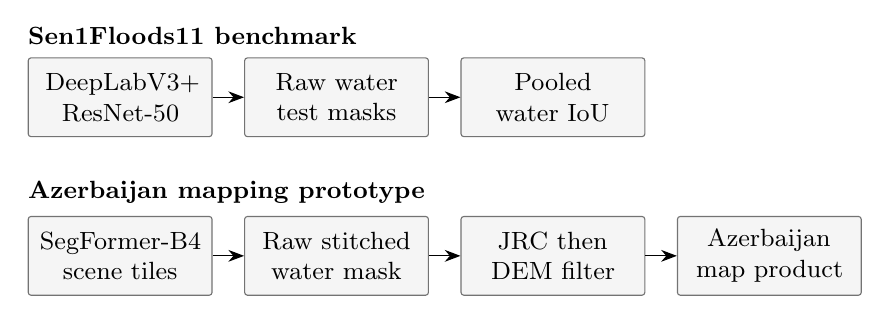
\begin{tikzpicture}[
  node distance=3mm and 4mm,
  stage/.style={draw=black!55, fill=black!4, rounded corners=1pt,
    align=center, font=\small, minimum height=10mm, text width=21mm},
  every edge/.style={draw, -{Stealth[length=2mm]}},
]
\node[stage] (study) {DeepLabV3+\\ResNet-50};
\node[stage,right=of study] (test) {Raw water\\test masks};
\node[stage,right=of test] (iou) {Pooled\\water IoU};
\node[anchor=south west,inner sep=0pt,font=\small\bfseries] at
  ([yshift=1.5mm]study.north west) {Sen1Floods11 benchmark};
\path (study) edge (test) (test) edge (iou);
\node[stage,below=10mm of study] (model) {SegFormer-B4\\scene tiles};
\node[stage,right=of model] (raw) {Raw stitched\\water mask};
\node[stage,right=of raw] (filter) {JRC then\\DEM filter};
\node[stage,right=of filter] (map) {Azerbaijan\\map product};
\node[anchor=south west,inner sep=0pt,font=\small\bfseries] at
  ([yshift=1.5mm]model.north west) {Azerbaijan mapping prototype};
\path (model) edge (raw) (raw) edge (filter) (filter) edge (map);
\end{tikzpicture}

\caption{Benchmark and prototype paths. Both use VV, VH and VV$-$VH.
Water IoU for the event-held-out comparison is computed on raw
DeepLabV3+ output. The Azerbaijan prototype filters the raw stitched
SegFormer-B4 water mask with JRC occurrence and DEM-based terrain and
coverage information before rendering the map.}
\label{fig:pipeline}
\end{figure}

\subsection{Input Representation}
\label{sec:input}

The network input is a three-channel SAR image of size $512\times512$
with the channels VV (vertical--vertical), VH (vertical--horizontal),
and their ratio, computed as the difference VV$-$VH in dB. The
polarizations are complementary. VV carries the surface backscatter,
and VH helps to separate land from water, because smooth water
backscatters much less than surrounding land. The ratio channel emphasizes
the difference between the two polarizations. Using three channels also
matches the input format expected by ImageNet-pretrained encoders
\cite{deng2009}, so the pretrained first layer can be used without
modification.

Each channel is clipped to a fixed dB range and then linearly rescaled to
$[0,1]$: VV to $[-25,0]$ dB, VH to $[-35,0]$ dB, and VV$-$VH to
$[0,18]$ dB. The exploratory analysis used to set these ranges drew from
the full hand catalog. Its reconstructed 80-chip sample includes 16
official test SAR inputs, three Bolivia holdout inputs and all 11
hand-labeled groups. The fixed ranges were shared by both comparison
arms and incorporate benchmark test covariates.

Wind roughens the water surface and raises its backscatter, so water can
resemble land. Conversely, recurrent water and radar shadow can both
look dark. This motivates the two downstream exclusions in
Sec.~\ref{sec:fusion}.

\subsection{Architecture}

We use DeepLabV3+ \cite{chen2018deeplabv3plus} with an ImageNet-initialized
ResNet-50 encoder \cite{he2016resnet} for the event comparison.
DeepLabV3+ is an encoder--decoder architecture for semantic segmentation.
Dilated convolutions and an Atrous Spatial Pyramid Pooling (ASPP) module
capture context at multiple scales, and a lightweight decoder refines
the result to sharpen object boundaries.

\subsection{Two-Stage Training}
\label{sec:training}

Hand-labeled data are scarce, so we train in two stages: pretraining
on chips whose labels were derived automatically from Sentinel-2 imagery,
followed by fine-tuning on manually annotated chips. The first stage
exposes the model to a large but noisy dataset, and the second adapts it
to expert labels. The named held-out event is excluded from both stages
in the reconstructed LOCO manifests (Sec.~\ref{sec:protocol}). We compare
with a single-stage baseline trained on hand labels in
Sec.~\ref{sec:ablations}.

\paragraph{Optimization.}
Both stages use Adam with a constant learning rate and no weight decay
or scheduler, and Dice loss except where noted. The effective batch
size is 8 (batch size 2 with 4 gradient-accumulation steps), and training
uses mixed precision (fp16). Pretraining uses a learning rate of
$3\times10^{-4}$ for up to 20 epochs with early stopping (patience 5).
Fine-tuning uses $10^{-4}$ for up to 50 epochs, keeping the checkpoint
with the best validation IoU. Training augmentation is horizontal flip,
vertical flip and right-angle rotation, each applied independently
with probability 0.5. Validation and test chips are not augmented.

\subsection{Loss Function}

With water in roughly one in ten labeled training pixels, the loss must
cope with strong class imbalance. We compared 11 variants, including
binary cross-entropy (BCE) with positive weights of 1, 4, 8.4 and 13,
and overlap-based objectives. We adopt the Dice loss \cite{milletari2016},
shown without its numerical stabilizer:
\begin{equation}
\mathcal{L}_{\mathrm{Dice}}
=1-\frac{2\sum_i p_i g_i}{\sum_i p_i+\sum_i g_i},
\label{eq:dice}
\end{equation}
where $p_i\in[0,1]$ is the predicted water probability and
$g_i\in\{0,1\}$ the label on valid pixel $i$. Dice was within 0.001
validation IoU of the leading Tversky variant in the short ResNet-34
sweep, and needs no additional class-imbalance hyperparameter
(Sec.~\ref{sec:ablations}).

\subsection{Post-Processing Fusion}
\label{sec:fusion}

\paragraph{Recurrent water (JRC).}
We use JRC Global Surface Water occurrence \cite{pekel2016high} and
subtract predicted positives where valid historical occurrence is at
least 20\%. This threshold is a recurrence proxy. It can remove genuine
event-date water as well as persistent water. Missing JRC pixels trigger
no JRC exclusion.

\paragraph{Layover and shadow (DEM).}
Radar terrain distortions depend on the viewing geometry and local
slope \cite{vollrath2020}. On a north-up raster, columns increase
eastward and rows increase southward. Let $s$ be the terrain slope
magnitude and $\alpha$ the downhill aspect, clockwise from north.
The sensor-to-ground azimuth $\varphi$ is nominally $90^\circ$ for
ascending passes and $270^\circ$ for descending passes. For nominal
incidence $\theta_i$, the signed angle in the range plane is
\begin{equation}
\theta_{\mathrm{loc}}=\theta_i+
\arctan\!\bigl(\tan s\cos(\varphi-\alpha)\bigr).
\label{eq:local-incidence}
\end{equation}
Terrain rising along the look direction faces the sensor. Its
downhill projection along that direction is negative, reducing
local incidence. Pixels with $\theta_{\mathrm{loc}}\leq0^\circ$ are
flagged for layover and those with $\theta_{\mathrm{loc}}\geq90^\circ$
for shadow. Both scene replays use SRTM1 \cite{farr2007}, a nominal
incidence of $37.55^\circ$ (the midpoint of $29.1^\circ$ and $46.0^\circ$),
and the eastward look approximation. Missing DEM is excluded along
with a one-pixel dilation of the coverage gaps.

\paragraph{Order of operations and evaluation.}
The JRC mask is subtracted from predicted water first, and the
terrain/coverage mask is applied second. Sen1Floods11 labels include
persistent water present on the event date, so the benchmark scores raw
water masks before these exclusions. We examine the filtered map as a
separate downstream product in Sec.~\ref{sec:deployment}.

\section{Experiments}
\label{sec:experiments}

\subsection{Setup}

Section~\ref{sec:dataset} describes the data, protocol and metrics.
Section~\ref{sec:method} describes the model, optimizer, batch size
and augmentation. We found no canonical chip-ID overlap between the
official test subset and the reconstructed weak or hand training and
validation roles. The georeferenced checks likewise found no positive-area
interior intersections above the specified tolerance ($10^{-8}$ degrees
on both axes) across 425,250 generalist test-to-role tile pairs. Boundary
contacts or sub-tolerance intersections occur for 73 test chips against
weak training and 35 against hand training. These checks describe the
recorded membership and current raster grids. Shared scene context,
adjacency and preprocessing exposure remain sources of dependence.

\subsection{LOCO Results}
\label{sec:loco}

Table~\ref{tab:a1test} reports the nine recoverable event--seed comparisons
out of 30 planned, spanning seven events and 51 of the 90 unique
official test chips. The fixed generalist reaches pooled IoU 0.676564
and F1 0.807084 over all 90 chips. Two official chips contain no valid
pixels and contribute zero counts. Ghana, India and Paraguay have no
recoverable LOCO results under the frozen selection.

\begin{table}[!htbp]
\caption{Pooled water-class IoU on each event's official test chips.
Dashes indicate unavailable event-excluded results. Differences use
full-precision scores.}
\label{tab:a1test}
\centering\small
\begin{tabular}{@{}lrrrrr@{}}
\toprule
Event & Test chips & Seed & Generalist & LOCO & $\Delta$ \\
\midrule
Ghana & 11 & -- & 0.5793 & -- & -- \\
India & 14 & -- & 0.6655 & -- & -- \\
Mekong & 6 & 43 & 0.8443 & 0.8487 & $+0.0044$ \\
Mekong & 6 & 44 & 0.8443 & 0.8377 & $-0.0066$ \\
Nigeria & 4 & 43 & 0.8831 & 0.8912 & $+0.0080$ \\
Pakistan & 6 & 43 & 0.2690 & 0.2354 & $-0.0336$ \\
Pakistan & 6 & 44 & 0.2690 & 0.2943 & $+0.0253$ \\
Paraguay & 14 & -- & 0.6641 & -- & -- \\
Somalia & 6 & 42 & 0.5027 & 0.5151 & $+0.0124$ \\
Spain & 6 & 42 & 0.7237 & 0.7215 & $-0.0022$ \\
Sri Lanka & 9 & 42 & 0.8353 & 0.8377 & $+0.0024$ \\
USA & 14 & 42 & 0.5525 & 0.5522 & $-0.0003$ \\
\bottomrule
\end{tabular}

\end{table}

For USA seed 42, the historical evaluator used an interrupted run's
\texttt{best.ckpt}. The reconstruction uses the completed retry's
\texttt{best-v1.ckpt}, selected by its validation maximum. The two USA
scores consequently refer to different checkpoints. No all-event mean,
event ranking or three-seed interval is estimated from the surviving
runs.

\subsection{Interpolation vs. Generalization on Paired Test Chips}
\label{sec:sensitivity}

On the same test chips, five of the nine differences in Eq.~\ref{eq:paired} are positive
and four are negative, from $-0.033583$ to $+0.025312$.
Mekong and Pakistan each change sign between seeds 43 and 44.
Variation across generalist training runs remains unmeasured.

We recompute the difference after dropping each test chip in turn
from both models, leaving the weights, valid masks and threshold fixed.
Across 63 such omissions, seven of nine comparisons can reverse sign.
In Pakistan seed 44, one chip contains 171,908 of 198,897 labeled water
pixels. Removing that chip changes the difference from $+0.0253$ to
$-0.2220$. Figure~\ref{fig:chip-sensitivity} shows the full-chip
difference and the observed minimum and maximum under each single-chip
omission. These are deterministic sensitivity ranges on the observed
sample. They have no confidence-interval interpretation.

\begin{figure}[!htbp]
\centering
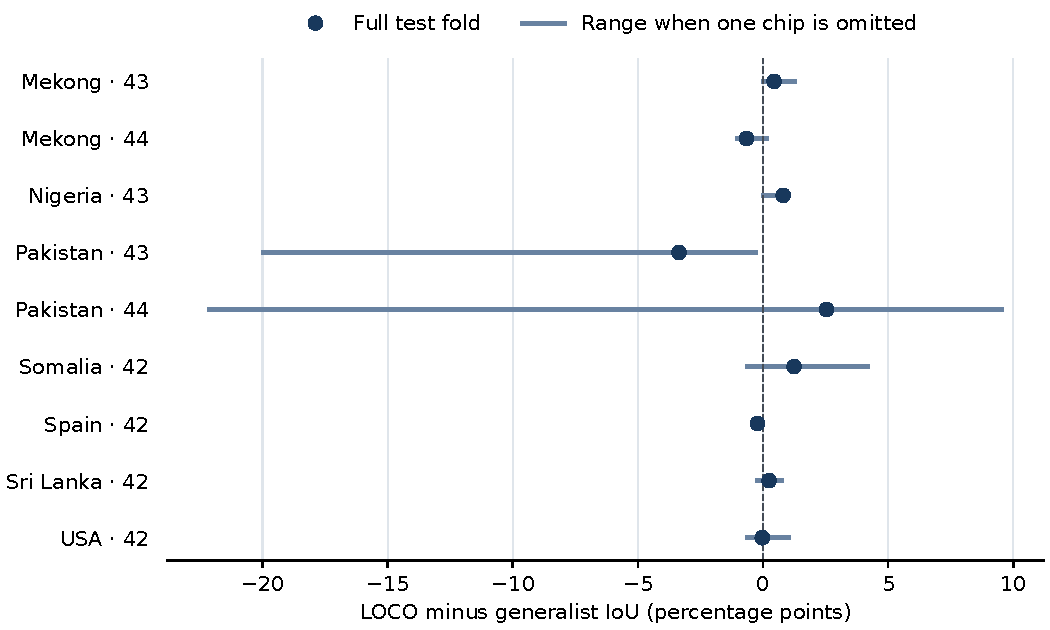
\includegraphics[width=\linewidth]{figures/chip_sensitivity.pdf}
\caption{Full-test paired water-IoU differences (dots) and the observed
minimum and maximum after omitting one test chip from both models
(horizontal ranges). The dashed line marks zero.}
\label{fig:chip-sensitivity}
\end{figure}

\subsection{Ablations}
\label{sec:ablations}

\paragraph{Two-stage training.}
We compare the two-stage scheme with a single-stage baseline trained
on hand labels only (Table~\ref{tab:two-stage}). These two seed-42
DeepLabV3+/ResNet-50 runs reached test IoUs of 0.6732 and 0.6766.
The fine-tuning settings recorded for the two runs were closely
matched, with different source snapshots. Weak labels provide a
greater variety of scenes than manual chips alone, a motivation for
pretraining. The numerical difference describes these two fits.

\begin{table}[!htbp]
\caption{Two-stage and hand-only DeepLabV3+/ResNet-50 runs, seed 42,
evaluated on the standard hand test split.}
\label{tab:two-stage}
\centering\small
\begin{tabular}{@{}lrr@{}}
\toprule
Training & IoU & F1 \\
\midrule
Single-stage (hand labels only) & 0.6732 & 0.8047 \\
Two-stage (weak $\to$ hand) & 0.6766 & 0.8071 \\
Difference & +0.0034 & +0.0024 \\
\bottomrule
\end{tabular}

\end{table}

\paragraph{Loss function.}
Table~\ref{tab:loss} gives the full sweep over 11 variants. The three
overlap-based losses (Focal-Tversky, Tversky and Dice) are within 0.001
validation IoU of each other. In this sweep their advantage over the
best BCE setting is about 0.04 IoU. Dice needs no imbalance
hyperparameter, which motivated its use in the event-held-out recipe.
BCE at weight 8.4, taken from the full-catalog label ratio, scored below
weight 4. The class-ratio heuristic was therefore a poor guide to the
best weight in this setting.

\begin{table}[!htbp]
\caption{Loss sweep on the 89-chip validation split using
DeepLabV3+/ResNet-34, seed 42, one run per variant on a Colab T4,
with a 40-epoch limit and early stopping (patience 8).}
\label{tab:loss}
\centering\small
\begin{tabular}{@{}lrr@{}}
\toprule
Loss & Val. IoU & Val. F1 \\
\midrule
Focal-Tversky ($\gamma=1.33$) & 0.6434 & 0.7830 \\
Tversky ($\alpha=0.3$, $\beta=0.7$) & 0.6427 & 0.7825 \\
Dice & 0.6425 & 0.7824 \\
Dice + Focal & 0.6261 & 0.7701 \\
Dice + BCE (weight 8.4) & 0.6066 & 0.7551 \\
BCE, positive weight 4 & 0.5988 & 0.7491 \\
BCE, positive weight 8.4 & 0.5525 & 0.7118 \\
Focal ($\alpha=0.25$) & 0.5428 & 0.7037 \\
Lov\'asz & 0.5136 & 0.6787 \\
BCE, positive weight 13 & 0.5107 & 0.6761 \\
BCE, positive weight 1 & 0.4749 & 0.6440 \\
\bottomrule
\end{tabular}

\end{table}

\section{Deployment in Azerbaijan}
\label{sec:deployment}

Azerbaijan has no coverage in Sen1Floods11, which motivated a local
mapping prototype. This section describes the prototype, which uses a
different segmentation model and has different evidence from the
event-held-out study.

\subsection{Production Model}

The prototype uses SegFormer-B4 \cite{xie2021segformer} with the
\texttt{nvidia/mit-b4} backbone and ImageNet initialization. It follows
the two-stage training scheme of Sec.~\ref{sec:training}. The logged best
weak-pretraining validation IoU was 0.658. On the hand split the selected
checkpoint reached a validation IoU of 0.7024, test IoU of 0.7027 and
test F1 of 0.8254. Checkpoints within each run were selected by
validation IoU. The historical choice of the default deployment
variant also used test IoU. The
\href{https://github.com/AliAgabalayev/Flood-Damage-Detection/commit/5e727aaed7b5995c6edeec33e90c4e8a87718c8f}{configuration history}
records that two B4 variants had higher validation scores, but the
default B4 beat both variants and the DeepLabV3+ generalist on test
IoU. Table~\ref{tab:model-comparison} records those benchmark runs for
the default and the same generalist as in Table~\ref{tab:two-stage}.
The test contrast is descriptive after model selection. It provides
no accuracy estimate for the Azerbaijan scenes.

\begin{table}[!htbp]
\caption{Logged results for two seed-42 runs on the standard
Sen1Floods11 hand split. These are raw water segmentation scores.}
\label{tab:model-comparison}
\centering\small
\begin{tabular}{@{}lrr@{}}
\toprule
Model & Val. IoU & Test IoU \\
\midrule
DeepLabV3+/ResNet-50 & 0.6712 & 0.6766 \\
SegFormer-B4 & 0.7024 & 0.7027 \\
\bottomrule
\end{tabular}

\end{table}

\subsection{Viewer and API}
\label{sec:api}

The web viewer covers five fixed sites with precomputed assets. It
offers layers for the map mask, recurrent water, model probabilities
and raw SAR, and exports PNG or GeoTIFF where available. A separate
upload page sends a GeoTIFF to the FastAPI \texttt{POST /predict}
endpoint. The model loads once at startup. Inference uses $512\times512$
tiles, 64-pixel overlap, feathered probability stitching and a threshold
of $\geq0.5$.

The revised upload path accepts north-up WGS~84 GeoTIFFs with at least
two bands. It aligns configured JRC and DEM data to the upload grid
and uses the nominal look geometry in Sec.~\ref{sec:fusion}. It
reports partial coverage and rejects requests with no jointly usable
reference coverage. On accepted uploads, missing DEM pixels and
their one-pixel boundary are excluded, while missing JRC values
cause no JRC subtraction. Area, scene percentage and the PNG overlay
come from the same final mask. The percentage uses the full raster as
its denominator.

On 25 November 2026, we sent the original Baku and Sabirabad
GeoTIFFs to a local server with the corrected terrain rule. Each returned HTTP 200 with partial
reference coverage. We decoded the overlay's alpha mask and compared
it pixel by pixel with a fresh offline CLI GeoTIFF using the same
checkpoint, inference settings and reference tiles
(Table~\ref{tab:api-replay}). Both overlays exactly matched the offline
masks. We checked the response bounds and recomputed the map statistics
from the decoded overlays. The final mapped areas were approximately
3.15~km$^2$ in Baku and 2.04~km$^2$ in Sabirabad.

\begin{table}[!htbp]
\caption{Corrected HTTP and CLI replay on the same raster grid.
HTTP and CLI water columns count positive pixels. The last two columns
count flips relative to the previous implementation, for terrain
exclusions and final water separately.}
\label{tab:api-replay}
\centering\small
\begin{tabular}{@{}lrrrrr@{}}
\toprule
Site & HTTP water & CLI water & API--CLI diff. & Terrain flips & Water flips \\
\midrule
Baku & 41,321 & 41,321 & 0 & 892 & 2 \\
Sabirabad & 26,668 & 26,668 & 0 & 0 & 0 \\
\bottomrule
\end{tabular}

\end{table}

\subsection{Scene Provenance}

The project records Baku on 7 April 2026 and Sabirabad on 30 June 2026
as Sentinel-1 GRD IW acquisitions with VV and VH, retrieved using
Google Earth Engine \cite{gorelick2017}. The archived rasters lack
original Sentinel product IDs and overpass times. The Baku City
Executive Power reported heavy rainfall and suburban flooding on
6 April \cite{baku2026}. This provides context for the acquisition.
The records examined for Sabirabad did not confirm a matching event.

\subsection{Reference Labels}

We found no independently labeled inundation extent aligned in time
and grid to either acquisition. Earlier before/after Baku masks were
on a different grid and lacked reliable acquisition and labeling
provenance. The municipal report concerns impacts at city scale and
does not delineate inundation on the radar grid. Both scenes are
treated as unlabeled mapping examples.

\subsection{Effect of Post-Processing}
\label{sec:map-effects}

Table~\ref{tab:deployment} shows the historical offline products and
the CPU replay with the archived exclusion masks. Each replay differs
from the corresponding archived final by one positive pixel. On these
scene grids the approximately mapped area changes from 73.08 to
3.15~km$^2$ in Baku and 8.94 to 2.04~km$^2$ in Sabirabad. The removed
fraction of raw positives is 95.7\% and 77.2\%, respectively. It measures
the effect of the filters on the prediction.

\begin{table}[!htbp]
\caption{Historical offline map products and replay using the archived
terrain rule. All values are positive pixel counts. The corrected replay
is reported separately in Table~\ref{tab:api-replay}.}
\label{tab:deployment}
\centering\small
\begin{tabular}{@{}llrrrr@{}}
\toprule
Site & Date & Raw & After JRC & Replay final & Archived final \\
\midrule
Baku & 2026-04-07 & 960,106 & 165,158 & 41,319 & 41,320 \\
Sabirabad & 2026-06-30 & 116,713 & 44,785 & 26,668 & 26,669 \\
\bottomrule
\end{tabular}

\end{table}

The archived terrain masks use the earlier sign convention, which
reversed the terrain projection in Eq.~(\ref{eq:local-incidence}).
SRTM1 at the nominal geometry reproduces those historical masks.
Dilated DEM gaps account for 1,240,996 of 1,241,953 archived flags in
Baku and all 1,826,806 in Sabirabad. A zero in the archived final
mask may indicate an exclusion or a negative prediction.

The corrected rule leaves these gap counts and the JRC masks
unchanged. In Baku it adds 47 and removes 845 terrain exclusions
outside the gaps, changing 892 terrain pixels. Only two final pixels
change relative to the prior inference on the same inputs, both
returning to the water mask. In Sabirabad, both masks are unchanged.
Relative to the archived final products, the corrected water maps
differ at three pixels in Baku and one in Sabirabad.


\subsection{Limitations}

Each Sen1Floods11 group represents a particular flood event and scene
context. The study measures transfer on the surviving models and
observed chips. The prototype uses a single nominal incidence angle
and local reference coverage, which strongly affects the resulting
map. The two unlabeled scenes leave false alarms, missed water and
the accuracy effect of filtering unmeasured. The reference tiles and
checkpoint used in local replay are listed in the reproducibility
package.

\section{Conclusion}
\label{sec:conclusion}

We revisited the distinction between within-event interpolation and
event-held-out generalization in SAR water segmentation. The corrected
comparison uses identical official test chips for each surviving
event-excluded checkpoint and a fixed generalist. On nine recoverable
event--seed pairs across seven events, five differences favored the
event-excluded checkpoint and four favored the generalist. Dropping
one chip could change the sign in seven pairs. This dependence on the
observed chips, together with incomplete seeds and different training
and validation sets, limits what the comparison says about new events.

The Azerbaijan prototype uses SegFormer-B4 and applies JRC occurrence
and terrain/coverage exclusions to the raw water masks. The two
historical scene products show how strongly those choices affect the
mapped extent, particularly where the DEM is missing. Accuracy in
Azerbaijan remains unmeasured. Repeated training on matched designs
and independent inundation labels at the satellite overpass would
address the benchmark and prototype limitations, respectively.

\paragraph{Code and reproducibility.}
The historical benchmark uses ML commit \texttt{867a4f3}. The upload
API and offline CLI use the
\href{https://github.com/AliAgabalayev/Flood-Damage-Detection/commit/23563a7bebf28e508b394cf6858649718fd148a3}{terrain-corrected ML commit}
(\texttt{23563a7}). The
\href{https://github.com/AliAgabalayev/flood-paper/tree/paper-v1.0}{companion manuscript repository}
provides archived per-chip confusion counts, scene replay records and
commands to regenerate the tables and figures.


\par\medskip
\noindent\textbf{License.} Copyright \copyright{} 2026 the authors.
Original manuscript text and author-created scholarly figures and tables are
licensed under \href{https://creativecommons.org/licenses/by/4.0/}{CC BY 4.0}.
Third-party material is excluded and retains its applicable terms.

\bibliographystyle{splncs04}
\bibliography{main}
\end{document}
